% ECIR 2027 -- SHORT PAPER
%
% Springer LNCS template (llncs.cls v2.25). Compliance notes:
%   Sec. 4.2  short papers are 6-11 pages.
%   Sec. 4.5  no colour anywhere; figures greyscale with distinct markers/hatching, vector PDF,
%             drawn at the true text width so no label falls below 6 pt.
%   Sec. 4.1  only two heading levels numbered.
%   Sec. 4.9  citations by number via splncs04.
%
% EVERY NUMBER IS \input{} FROM tables/, regenerated by build_artifacts.py from the run CSVs.
% Do not hand-edit a numeric table: change the experiment and rebuild. Numbers quoted inline are
% cross-checked against data/facts_7d.txt, which the same script writes.
%
% NAMING: strategies are named, not lettered -- Fresh, Wait, Reweight, Correct, Twice, Distil, plus
% the infeasible Oracle. Registry keys (DISTILL_T, ULC, ...) are internal and must not appear.
%
% IP BOUNDARY: industrial motivation rests only on the public Meta GEM engineering post and on
% textbook auction mechanics. No internal system names, roadmaps, architectures or numbers.
%
\documentclass[runningheads]{llncs}

\usepackage[T1]{fontenc}
%\usepackage{newtxtext}
%\usepackage[varvw]{newtxmath}
\usepackage{graphicx}
\usepackage{booktabs}
\usepackage{amsmath}
\usepackage{amssymb}
\usepackage{tikz}
\usetikzlibrary{arrows.meta, positioning, patterns}

\newcommand{\ind}{\mathbf{1}}
\newcommand{\Yo}{Y^{(o)}}
\newcommand{\Yv}{Y^{(v)}}

\begin{document}

\title{One Record per Click: Serving Capacity Selects the Training Target in Delayed-Feedback Conversion Prediction}
\titlerunning{One Record per Click}

\author{Anonymous Author\inst{1}}
\authorrunning{A. Author}
\institute{Anonymous Institution, Anonymous City, Country\\
\email{anonymous@example.org}}

\maketitle

\begin{abstract}
Many production conversion-rate (CVR) pipelines write exactly one training record per click: it is
emitted after a fixed wait $\Delta$, carries the label
$\ind[\text{conversion} \le \text{click}+\Delta]$, and is never revisited. We show that this
contract reduces the choice of training target to a one-dimensional design problem --- how much of
the target is a realised hard label and how much a model-produced soft one --- and that the served
model's capacity selects where on that axis to sit. Instrumenting the feature path of fourteen
published methods over a full 720-hour replay of the Criteo Delayed Feedback Dataset (Criteo-DFD),
we find that nine emit more than one record per click, including the \textsc{Vanilla} baseline the
field normalises against, so their reported gains are not attainable under the contract. Sweeping
target hardness over the admissible remainder against a five-rung serving-capacity ladder
($26$\,K--$9.6$\,M parameters) yields two ordered crossovers. At the smallest rung a purely soft
target that uses no realised label at all is the best arm, beating even the non-causal Oracle by
$0.0029$ area under the ROC curve (AUC); by $46$\,K the hybrid targets of prior work overtake it;
and beyond $10^{5}$ parameters the Oracle's true label is best, with the soft target now costing
$0.0084$. We further find that a published baseline's prescribed auxiliary
learning rate costs it $0.0022$ AUC, roughly seven times the gap between the methods it is used to
compare.
\keywords{Conversion rate prediction \and Delayed feedback \and Knowledge distillation
\and Online advertising.}
\end{abstract}

% =====================================================================================
\section{Introduction}
% =====================================================================================

Conversion-rate (CVR) prediction decides what an advertising system shows and what it charges, and
it is trained continuously on a stream. Its central difficulty is that the label arrives late: a
click is observed immediately, but the conversion it may cause can follow minutes, days or weeks
afterwards~\cite{chapelle2014modeling}, so a model trained on the labels observed so far is trained
on a censored, downward-biased target. The literature treats this as an estimation problem, and a
decade of work has produced importance
weighting~\cite{yasui2020feedback,yang2021capturing}, label
correction~\cite{chen2022asymptotically,wang2023unbiased}, duplicated replay
streams~\cite{ktena2019addressing,gu2021real,dai2023dually}, multi-window
ensembles~\cite{li2021follow,liu2024online,zhang2025personalized} and influence-function
retrofits~\cite{ding2026delayed}. Almost all share an unstated systems assumption: that a click may
be written into the training stream more than once --- re-emitted when its conversion lands,
replayed when its window closes, or relabelled at several horizons.

Many production pipelines cannot do this. A common contract is:

\begin{quote}
A click produces \emph{exactly one} training example. It is emitted after a fixed wait $\Delta$,
carries the label $\ind[\text{conv\_ts} \le \text{click\_ts} + \Delta]$, and is never revisited. If
the conversion has not arrived by then, the example is negative permanently.
\end{quote}

The reasons are mundane and therefore durable: amending a materialised example later means mutable
training data, duplicate-key handling, and a reproducibility story that breaks on every backfill,
whereas freezing the label at $\Delta$ keeps the dataset append-only and the pipeline replayable.
The contract is not our invention. It is the literal reading of the field's own reference baseline,
which ``trains each click \emph{once} at base observation age $o$''~\cite{li2026twice}. What we show
is that the implementations do not honour it --- including, as Sect.~\ref{sec:audit} establishes,
that baseline's own.

\smallskip\noindent\textbf{One record, one question.} The contract is restrictive enough to be
clarifying. If a click yields a single record carrying a single target, the only remaining freedom
is \emph{what that target says}. At one extreme it is a realised outcome: a hard $0/1$ draw,
unbiased but high-variance, and correct only for conversions fast enough to have landed. At the
other it is a model's estimate: a soft probability, lower-variance and defined for every record,
but capped by the estimator that produced it. Every admissible method is a point between these two.
\textsc{Fsiw}~\cite{yasui2020feedback} reweights the hard label,
\textsc{Ulc}~\cite{wang2023unbiased} blends it with a learned correction, and
\textsc{Twice}~\cite{li2026twice} routes the residual to a separate head. We call this quantity the
\emph{hardness} of the target, and we show that the best choice along it is not a property of the
dataset but of the \emph{served model's capacity} --- the axis a latency-bound ranker is actually
constrained on, and the one the delayed-feedback literature holds fixed.

\smallskip\noindent\textbf{Contributions.}
\begin{enumerate}
\item \textbf{A measurement, not an assertion.} We instrument the feature path of fourteen methods
and count training records per click over a full replay (Sect.~\ref{sec:audit}). Nine exceed one.
Two measurement traps --- traffic variation and window length --- both \emph{understate} violations;
we control for both.
\item \textbf{A reformulation.} Under the contract the admissible targets form a single hardness
axis spanned by two label pipelines (Sect.~\ref{sec:formulation}), and a purely soft target
satisfies the frozen-label obligation \emph{vacuously}, its record carrying no label to freeze
(Proposition~\ref{prop:axis}).
\item \textbf{The main result.} Optimal hardness increases with serving capacity, through two
ordered and significant crossovers (Sect.~\ref{sec:hardness}): the soft target cedes to the hybrid
between $26$ and $46$\,K parameters, and the hybrid cedes to the Oracle's true label near
$10^{5}$. Below that second crossing the non-causal Oracle is \emph{not} an upper bound.
\item \textbf{A reproducibility finding.} Baseline auxiliary learning rates do not transfer: one
baseline's prescribed rate costs it $0.0022$ AUC while the same change \emph{harms} another
(Sect.~\ref{sec:tuning}), so the admissible ordering cannot be read without per-method tuning.
\end{enumerate}

% =====================================================================================
\section{Related Work}\label{sec:related}
% =====================================================================================

We organise prior work by whether it can be expressed as one record per click, because that is what
the constraint decides. Sect.~\ref{sec:audit} gives measured counts; here we give the mechanism.

\smallskip\noindent\textbf{Methods that need more than one record.} The fake-negative family writes
the click as a negative and re-emits it as a positive when the conversion
arrives~\cite{ktena2019addressing}; \textsc{Es-Dfm} samples an elapsed-time cut-off and duplicates
the delayed positive~\cite{yang2021capturing}, \textsc{Defer} replays real negatives once their
window closes~\cite{gu2021real}, \textsc{Ddfm} runs both streams together~\cite{dai2023dually}, and
\textsc{Defuse} adds a label correction on top of the duplicated
stream~\cite{chen2022asymptotically}. Multi-window methods relabel the same click at several
horizons: \textsc{Ftp} trains $K$ maturity-gated tasks and a policy over
them~\cite{li2021follow}, \textsc{Miss} duplicates each delayed positive into every head's
stream~\cite{liu2024online}, and \textsc{Pi} interpolates two fixed-window
predictors~\cite{zhang2025personalized}. \textsc{If-Dfm} applies an influence-function update when
a label reverses~\cite{ding2026delayed}. In each case the extra visit \emph{is} the mechanism, not
an implementation detail that could be removed.

\smallskip\noindent\textbf{Single-record methods, and where they sit on the axis.} A smaller group
reweights or relabels the one fresh record, and these are what the constraint leaves standing.
\textsc{Fsiw} keeps the realised label and importance-weights the loss~\cite{yasui2020feedback};
\textsc{Ulc} adds a learned correction to it, giving a target that is part observation and part
estimate~\cite{wang2023unbiased}; \textsc{Twice} keeps its CVR tower on a single fresh record and
routes conversion-clock events to a separate delay head~\cite{li2026twice}. All three retain the
record's own realised label; none removes it. The end of the axis at which the target is a model
estimate alone is, to our knowledge, unmeasured in this literature, and Sect.~\ref{sec:hardness}
shows it is the best admissible choice at small serving capacity.

\smallskip\noindent\textbf{Distillation with privileged information.} Training-time-only signals
have been distilled into serving models before, notably privileged features at
Taobao~\cite{xu2020privileged}, and soft labels carry lower target variance than a hard Bernoulli
label~\cite{menon2021statistical} --- the mechanism we invoke in Sect.~\ref{sec:hardness}. The
privilege we exploit is neither a feature nor scale but \emph{time}: the estimator producing the
soft target is allowed to wait.

\section{Problem Formulation}\label{sec:formulation}
% =====================================================================================

\subsection{Notation and two clocks}

\begin{table}[t]
\caption{Notation. Times are absolute seconds; $o \ll v$ throughout}
\label{tab:notation}
\centering\small
\begin{tabular}{l l}
\toprule
symbol & meaning\\
\midrule
$x_i,\ C_i$ & features and click time of click $i$\\
$V_i,\ D_i = V_i - C_i$ & conversion time and delay ($D_i = \infty$ if no conversion)\\
$v$ & attribution window; the business-defined horizon of the served target\\
$o$ & base observation age: the shortest wait at which a record may be emitted\\
$\Delta$ & the pipeline's actual wait before emitting the record\\
$\Yv_i = \ind[D_i \le v]$ & the served target, knowable only at $C_i + v$\\
$\Yo_i = \ind[D_i \le o]$ & the label observable at emission when $\Delta = o$\\
$p_v(x) = P(\Yv{=}1 \mid x)$ & the estimand; a model of it is written $\hat p_v$\\
$w(x) = P(\Yv{=}1 \mid \Yo{=}0,\, x)$ & the residual correction shared by \textsc{Fsiw},
\textsc{Ulc}, \textsc{Es-Dfm}\\
$\tilde y_i$ & the target actually written on click $i$'s record\\
\bottomrule
\end{tabular}
\end{table}

Table~\ref{tab:notation} fixes notation. Following the long-horizon formulation
of~\cite{li2026twice}, clicks are observed on a \emph{click clock} and conversions arrive on a
separate \emph{conversion clock}: a business attribution window $v$ fixes the served target $\Yv$,
and training must predict $\Yv$ from a record written before $\Yv$ is known.

\subsection{The single-visit constraint}

Let $\Delta$ be the pipeline's wait. The contract of Sect.~1 imposes two obligations:
\begin{description}
\item[R1 (single visit)] click $i$ contributes exactly one training record, ever;
\item[R2 (frozen label)] that record's label is $\ind[D_i \le \Delta]$ for the $\Delta$ at which it
was emitted; no later-arriving conversion may add or change supervision.
\end{description}
A method may fail either independently: duplication fails R1, and reading $\Yv$ on a record released
before $C_i + v$ fails R2.

\subsection{Two label pipelines}

Because a record is written once and $\Delta$ is the only free quantity, the constraint admits
exactly two useful pipelines over the same clicks:
\begin{align}
\mathcal{D}_{\text{fresh}} &= \{(x_i,\, \Yo_i)\},\ \ \Delta = o \ll v
  &&\text{timely, biased low,}\\
\mathcal{D}_{\text{mat}} &= \{(x_i,\, \Yv_i)\},\ \ \Delta = v
  &&\text{unbiased, stale by } v .
\end{align}
For $\mathcal{D}_{\text{fresh}}$, $\mathbb{E}[\Yo \mid x] = p_v(x)\,F(o \mid x) < p_v(x)$, so it is
biased low by exactly the fraction of converters not yet observed. On Criteo-DFD at $o=1$\,h that
fraction is $0.77$, $0.57$ and $0.47$ at $v=1$, $7$ and $30$\,d: censoring deepens as the window
lengthens, yet even at $v=30$\,d the fresh label still carries almost half the target's positives,
which makes this corpus a conservative setting for any method that discards it.
$\mathcal{D}_{\text{mat}}$ carries the true target but its most recent row is $v$ old.

R1 forbids training the served model on both. What remains is to write one record at $\Delta = o$
and use $\mathcal{D}_{\text{mat}}$ to shape \emph{what its target says}.

\subsection{The target-hardness axis}\label{sec:axis}

Every admissible target is a function of the record's own realised label $\Yo_i$ and of quantities
estimated on $\mathcal{D}_{\text{mat}}$. Writing the general single-record form
\begin{equation}\label{eq:family}
\tilde y_i \;=\; \Yo_i\,\alpha(x_i) \;+\; \bigl(1 - \Yo_i\bigr)\,\beta(x_i),
\end{equation}
with $\alpha,\beta$ fitted on $\mathcal{D}_{\text{mat}}$ and frozen at emission, gives a
one-dimensional family ordered by how much the target depends on the realised label. We name three
points on it, and they are the arms we compare:
\begin{description}
\item[hard] the target \emph{is} a realised label: $\alpha{=}1,\beta{=}0$ recovers
$\tilde y = \Yo$ (\textsc{Fresh}); the non-causal reference $\tilde y = \Yv$ (\textsc{Oracle}) lies
outside the family, since $\Yv$ is not knowable at $\Delta = o$;
\item[hybrid] realised label plus a learned correction: $\alpha{=}1,\beta{=}w$ gives
$\tilde y = \Yo + (1-\Yo)w(x)$, which is exactly \textsc{Ulc}~\cite{wang2023unbiased};
\item[soft] a model estimate alone: $\alpha{=}\beta{=}\hat p_v$ gives $\tilde y = \hat p_v(x)$,
which uses no realised label at all.
\end{description}
\textsc{Fsiw}~\cite{yasui2020feedback} sits at the hard end by a different route, leaving
$\tilde y = \Yo$ and reweighting the loss instead of the target.

\begin{proposition}\label{prop:axis}
Let $\tilde y_i$ follow \eqref{eq:family} with $\alpha,\beta$ fitted on $\mathcal{D}_{\emph{mat}}$
and frozen at emission time $C_i + o$. Then \emph{(i)} $\tilde y_i$ is computable at $\Delta = o$
and the record satisfies \emph{R1} and \emph{R2}; and \emph{(ii)} if $\alpha \equiv \beta$, the
record satisfies \emph{R2} \emph{vacuously}: its target is a function of $x_i$ alone, so it carries
no realised label that a later-arriving conversion could revise.
\end{proposition}

\begin{proof}
(i) The record is written once, at $\Delta = o$, so R1 holds. Its target is a deterministic function
of $(x_i, \Yo_i)$ and of parameters frozen at emission; $\Yo_i$ is knowable at $C_i + o$ and is
never revised, so R2 holds. (ii) If $\alpha \equiv \beta$ then \eqref{eq:family} collapses to
$\tilde y_i = \alpha(x_i)$, which does not depend on $\Yo_i$. R2 constrains the realised label
carried by the record, and there is none. \qed
\end{proof}

Proposition~\ref{prop:axis}(ii) is the structural reason to care about the soft end beyond accuracy:
a record with no realised label needs no label join on the timely path. We return to this in
Sect.~\ref{sec:discussion}.

% =====================================================================================
\section{Instantiating the Axis}\label{sec:method}
% =====================================================================================

Realising the hybrid and soft points of Sect.~\ref{sec:axis} requires an estimator of $w$ and of
$p_v$ that is itself admissible. We fit one model on the matured pipeline and read both from it, so
that a comparison across the axis changes the target and nothing else.

The estimator trains only on clicks whose window has closed, $C_i + v \le T_n$ at cutoff $T_n$,
under the true label $\Yv$. It is causal by construction --- every training row's outcome was
knowable at $T_n$ --- and is itself R1/R2-compliant at $\Delta = v$. It carries two read-outs on one
trunk:
\begin{equation}
\hat p_v(x) = P(\Yv = 1 \mid x),
\qquad
w^{T}(x) = P(\Yv = 1 \mid \Yo = 0,\, x).
\label{eq:heads}
\end{equation}
The second is the estimand the field shares --- it is \textsc{Ulc}'s $w$, \textsc{Es-Dfm}'s
delayed-positive rate and \textsc{Ddfm}'s $z_1$. Substituting \eqref{eq:heads} into
\eqref{eq:family} gives the two admissible arms we sweep: the hybrid
$\tilde y = \Yo + (1-\Yo)\,w^{T}(x)$, and the soft $\tilde y = \hat p_v(x)$. Because the estimator
is training-only it is unbound by the serving budget; that asymmetry is what buys the right to wait.

Two implementation points matter and are easy to get wrong; both cost us a run before they were
fixed. First, the estimator's learning rate must be \emph{decoupled} from the served model's:
sharing it makes a per-arm sweep tune two models with one scalar, which cost $0.0065$ AUC when it
happened to \textsc{Fsiw}'s auxiliary in our harness. Second, both read-outs must be withheld until
the estimator has seen a minimum number of matured rows --- the hybrid falling back to
$\tilde y = \Yo$ and the soft arm likewise --- because a zero-initialised head asserts $0.5$ on
every row, and a constant target yields a loss of $\ln 2$ at every learning rate. Without the guard
the soft arm's rate is selected on a degenerate objective; Sect.~\ref{sec:limits} records the one
window where this bites even with the guard in place.

% =====================================================================================
\section{Experiments}\label{sec:experiments}
% =====================================================================================

\subsection{Setup}\label{sec:setup}

\noindent\textbf{Dataset and protocol.} Criteo-DFD~\cite{chapelle2014modeling}, 60 days of clicks
with conversion timestamps. We follow the streaming replay of~\cite{li2026twice}: pre-train on days
$[0,30)$, then stream $[30,60)$ with hourly cut-offs; at each cut-off a model consumes the records
released in that hour and then predicts every click of the next hour exactly once, scored
retrospectively against $\Yv$. Base observation age $o = 1$\,h. We report $v = 7$\,d in the main
text and $v = 1$\,d as a second window.

\noindent\textbf{Evaluation metrics.} Area under the ROC curve (AUC) is the headline metric, with
area under the precision--recall curve (PR-AUC) and log-loss (LL) reported at the capacity-matched
rung. All numbers are means over five seeds, and every comparison is a paired $t$-test over matched
seeds ($^{\ast}p<0.05$, $^{\ast\ast}p<0.01$).

\noindent\textbf{Compared methods.} Table~\ref{tab:hardness} names every arm and its point on the
axis. \textsc{Reweight} is \textsc{Fsiw}~\cite{yasui2020feedback}, \textsc{Correct} is
\textsc{Ulc}~\cite{wang2023unbiased}, \textsc{Wait} trains on $\mathcal{D}_{\text{mat}}$ only, and
\textsc{Distil} and \textsc{Soft} use the estimator of Sect.~\ref{sec:method}. \textsc{Vanilla},
\textsc{Es-Dfm}~\cite{yang2021capturing}, \textsc{Defuse}~\cite{chen2022asymptotically} and
\textsc{Ddfm}~\cite{dai2023dually} are shown for reference but are inadmissible
(Sect.~\ref{sec:audit}). The non-causal Oracle labels the fresh record with $\Yv$.

\noindent\textbf{Implementation details.} Minibatch $8192$, AdamW, and a learning rate selected
\emph{per arm and per capacity} from
$\{10^{-6}, 2.5{\times}10^{-6}, 10^{-5}, 5{\times}10^{-5}, 2{\times}10^{-4}, 5{\times}10^{-4},
10^{-3}\}$ on a held-out chronological slice of the pre-training period. The served model is swept
over five rungs S0--S4 varying the categorical hash-table size ($36 \to 131{,}072$ rows, $26$\,K
$\to 9.6$\,M parameters) at a fixed embedding dimension of~8, so the ladder is a pure
serving-capacity axis. The matured-data estimator is held at $9.5$\,M parameters throughout. At S4
the served model and the estimator are within $1.3\%$ of the same parameter count, which is the
cleanest available control for capacity transfer. Auxiliary learning rates are swept per method for
the reason established in Sect.~\ref{sec:tuning}.

% -------------------------------------------------------------------------------------
\subsection{RQ1: which methods can be run at all?}\label{sec:audit}
% -------------------------------------------------------------------------------------

\begin{table}[t]
\caption{Training records per click, measured over a full 720-hour replay at $v=7$\,d. Counts are
per \emph{distinct click touched}, so traffic variation cannot inflate them, and the window covers
every method's longest revisit lag. $^{\dag}$\textsc{Twice}'s served tower is single-visit; its
delay head reads the conversion clock}
\label{tab:compliance}
\centering\small
\begin{tabular}{l r@{\hskip 1.1em} r@{\hskip 1.4em} c@{\hskip 1.0em} c}
\toprule
method & records/click & max & R1 & R2\\
\midrule
\multicolumn{5}{l}{\emph{admissible}}\\
\quad Fresh & 1.00 & 1 & \checkmark & \checkmark\\
\quad Wait / teacher & 1.00 & 1 & \checkmark & \checkmark\\
\quad Reweight & 1.00 & 1 & \checkmark & $\times$\\
\quad Correct & 1.00 & 1 & \checkmark & $\times$\\
\quad Twice & 1.00 & 1 & \checkmark & \checkmark$^{\dag}$\\
\midrule
\multicolumn{5}{l}{\emph{inadmissible}}\\
\quad Vanilla & 1.08 & 2 & $\times$ & $\times$\\
\quad DFM & 1.34 & 8 & $\times$ & $\times$\\
\quad ES-DFM & 1.08 & 2 & $\times$ & $\times$\\
\quad DEFUSE & 1.08 & 2 & $\times$ & $\times$\\
\quad DDFM & 1.89 & 2 & $\times$ & $\times$\\
\quad PI & 2.00 & 2 & $\times$ & $\times$\\
\quad MISS & 2.05 & 3 & $\times$ & $\times$\\
\quad IF-DFM & 2.90 & 99 & $\times$ & $\times$\\
\quad FTP & 3.00 & 3 & $\times$ & $\times$\\
\bottomrule
\end{tabular}

\end{table}

Table~\ref{tab:compliance} reports the measurement. We instrument the feature path of every arm and
count training records over a full 720-hour replay, charging only gradient-carrying forwards so
that merely \emph{scoring} a historical click is not counted. Two traps had to be controlled, and
ignoring either understates violations.\footnote{\emph{Traffic}: per-hour ratios conflate
duplication with diurnal variation, since a maturity-gated stream reads clicks from $v$ ago when the
rate differed; \textsc{Pi} scores a spurious $12.2$ that way. We divide by \emph{distinct clicks
touched}. \emph{Window}: over 48\,h \textsc{Pi} measures $1.00$, its two visits being $10.5$ days
apart. We run the full stream and score only clicks whose entire revisit horizon fits inside it.}

Nine of fourteen methods exceed one record per click. Two counts are exact integers and confirm the
instrument: \textsc{Pi} emits $2.00$, one per fixed-window head, and \textsc{Ftp} $3.00$, one per
task plus its prophet. \textsc{If-Dfm} touches one click up to 99 times. Only \textsc{Fsiw},
\textsc{Ulc} and \textsc{Twice} keep the served model single-visit.

\smallskip\noindent\textbf{The field's anchor is inadmissible.} \textsc{Vanilla} --- ``each click
trained once at base observation age $o$'' --- measures $1.08$ records per click, because matching
any published \textsc{Vanilla} row requires also emitting the late conversion as a
positive.\footnote{The fresh record alone predicts $0.107$ against a $0.227$ base rate and cannot
reproduce any published \textsc{Vanilla} log-loss; the reading that does is fresh label plus a
positive for conversions arriving after $o$.} Relative improvement reported against it is therefore
normalised by a baseline a single-visit pipeline cannot run.

\smallskip\noindent\textbf{On auxiliaries.} \textsc{Fsiw}, \textsc{Ulc} and \textsc{Twice} emit one
record for the served model but fit a \emph{separate} model on matured data, so they satisfy R1 and
sit at the boundary of R2. We read the constraint as governing the served model's training
pipeline, under which they comply; the alternative reading --- that no later-arriving conversion
may inform anything --- leaves only \textsc{Wait} standing and declares the problem unsolvable
rather than selecting a method. We adopt the former and say so, because the choice determines which
methods are admissible. Every arm we compare sits at exactly this level and no lower.

% -------------------------------------------------------------------------------------
\subsection{RQ2: is the admissible ordering readable?}\label{sec:tuning}
% -------------------------------------------------------------------------------------

Before comparing targets we must establish that the comparison is about targets. Each single-record
baseline prescribes a fixed learning rate for its auxiliary, and these are not interchangeable.
Holding everything else fixed and moving \textsc{Correct}'s auxiliary from its prescribed
$10^{-3}$ to $5{\times}10^{-4}$ raises it by $+0.0005^{\ast}$, $+0.0004^{\ast\ast}$,
$+0.0002^{\ast}$, $+0.0002^{\ast\ast}$ and $+0.0022^{\ast\ast}$ across S0--S4. The same change
applied to \textsc{Reweight} \emph{harms} it, by $-0.0005^{\ast\ast}$, $-0.0004^{\ast\ast}$ and
$-0.0036^{\ast\ast}$ at S0, S2 and S3.

Two consequences follow. First, the effect is large relative to what it is used to measure: at S4
the tuning alone moves \textsc{Correct} by $0.0022$, roughly seven times the $0.0003$ that separates
it from \textsc{Distil} once both are tuned. A comparison at prescribed rates would have reported a
$0.0025$ method gap that is $88\%$ tuning. Second, because the same change helps one baseline and
hurts another, the bias is not systematic and cannot be removed by a global correction. We
therefore sweep auxiliary rates per method and report the tuned value for every arm; all numbers
below are tuned. We flag this rather than bury it because it bounds how finely published orderings
in this literature can be read.

% -------------------------------------------------------------------------------------
\subsection{RQ3: optimal target hardness tracks serving capacity}\label{sec:hardness}
% -------------------------------------------------------------------------------------

\begin{figure}[t]
\centering
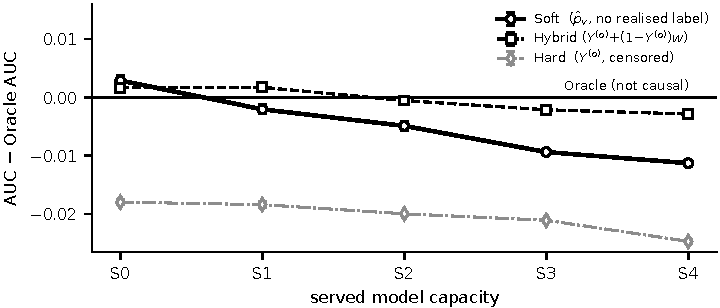
\includegraphics[width=\textwidth]{figs/fig_hardness_7d.pdf}
\caption{Both crossovers, plotted as a margin against the non-causal Oracle so that the Oracle is
the zero line; bars are 95\% intervals over five paired seeds. The soft and hybrid targets cross
\emph{each other} between S0 and S1, and both cross \emph{zero} between S1 and S2: below roughly
$10^{5}$ served parameters an estimated target beats the true one}
\label{fig:hardness}
\end{figure}

\begin{table}[t]
\caption{AUC against serving capacity, $v=7$\,d, five seeds, arms grouped by their point on the
hardness axis of Sect.~\ref{sec:axis}. Bold marks the best \emph{admissible} arm per column; the
Oracle is not causal and the inadmissible block cannot be run at all, so neither competes for it.
The bold entry moves from the soft target at S0 to the hybrid from S1 on}
\label{tab:hardness}
\centering\small
\begin{tabular}{lrrrrr}
\toprule
training target & S0 & S1 & S2 & S3 & S4\\
served parameters & 26K & 46K & 115K & 645K & 9.6M\\
\midrule
\multicolumn{6}{l}{\emph{hard: target is a realised label}}\\
\quad \textsc{Fresh}\ ($\tilde y = \Yo$) & 0.8077 & 0.8127 & 0.8182 & 0.8227 & 0.8218\\
\quad \textsc{Reweight}\ (loss-weighted $\Yo$) & 0.8218 & 0.8269 & 0.8334 & 0.8388 & 0.8396\\
\quad \textsc{Wait}\ ($\tilde y = \Yv$, stale by $v$) & 0.8105 & 0.8156 & 0.8212 & 0.8286 & 0.8321\\
\multicolumn{6}{l}{\emph{hybrid: realised label $+$ learned correction}}\\
\quad \textsc{Twice} & 0.8120 & 0.8217 & 0.8260 & 0.8305 & 0.8327\\
\quad \textsc{Correct} & 0.8281 & 0.8325 & 0.8374 & 0.8414 & 0.8434\\
\quad \textsc{Distil} & 0.8273 & \textbf{0.8328} & \textbf{0.8377} & \textbf{0.8416} & \textbf{0.8437}\\
\multicolumn{6}{l}{\emph{soft: model estimate alone, no realised label}}\\
\quad \textsc{Soft}\ ($\tilde y = \hat p_v$) & \textbf{0.8285} & 0.8291 & 0.8333 & 0.8344 & 0.8352\\
\midrule
\multicolumn{6}{l}{\emph{inadmissible: $>1$ record per click}}\\
\quad \textsc{Vanilla} & 0.8222 & 0.8280 & 0.8347 & 0.8403 & 0.8412\\
\quad \textsc{Es-Dfm} & 0.8166 & 0.8288 & 0.8357 & 0.8383 & 0.8421\\
\quad \textsc{Defuse} & 0.8171 & 0.8293 & 0.8362 & 0.8387 & 0.8423\\
\quad \textsc{Ddfm} & 0.8275 & 0.8314 & 0.8367 & 0.8412 & 0.8436\\
\midrule
\quad Oracle \emph{(not causal)} & 0.8256 & 0.8311 & 0.8382 & 0.8438 & 0.8465\\
\bottomrule
\end{tabular}

\end{table}

Table~\ref{tab:hardness} and Fig.~\ref{fig:hardness} are the main result, and the table is read
down the columns rather than across the rows: the best admissible target changes with capacity.

\smallskip\noindent\textbf{First crossover: soft cedes to hybrid between 26 and 46\,K parameters.}
At S0 the soft target is the best admissible arm, ahead of the hybrid by
$+0.0012^{\ast}$. By S1 the ordering has reversed, and it stays reversed and widens monotonically:
$-0.0038^{\ast\ast}$, $-0.0043^{\ast\ast}$, $-0.0072^{\ast\ast}$ and $-0.0084^{\ast\ast}$ at
S1--S4. The soft arm's own ladder is nearly flat ($0.8285 \to 0.8352$ across the five rungs) where
the hybrid's climbs ($0.8273 \to 0.8437$), which is the mechanism: a purely soft target is a
\emph{function of $x$}, so two records with identical features receive identical supervision, and a
larger model can only fit that function more exactly. The realised label carries per-example
information that no function of $x$ reproduces. A small model cannot exploit that information and
is hurt by its Bernoulli variance~\cite{menon2021statistical}; a large one can, and discarding it
becomes pure loss.

\smallskip\noindent\textbf{Second crossover: the Oracle is not an upper bound below $10^{5}$
parameters.} The hybrid beats the non-causal Oracle at S0 and S1, by $+0.0017^{\ast\ast}$ at both,
and loses from S2 on ($-0.0005^{\ast}$, $-0.0021^{\ast\ast}$, $-0.0029^{\ast\ast}$). The soft
target beats it more decisively still at S0, by $+0.0029^{\ast\ast}$. Below roughly $10^{5}$
parameters a corrected or estimated target is therefore \emph{better supervision than the true
label}, for the same variance reason. This matters for how the literature evaluates: an assessment
conducted only at large capacity reports a delayed-feedback penalty that a deployable model does
not fully pay.

\smallskip\noindent\textbf{Within the hybrid class, the source of the correction barely matters.}
\textsc{Distil} and \textsc{Correct} differ by $-0.0007$ to $+0.0004$ across the ladder, reaching
$p<0.05$ only at S3 and S4 and never exceeding $0.0003$ there. This is a parity result, and it is
informative: the two correctors hold the same parameter count to within $0.13\%$
($9{,}444{,}801$ against $9{,}456{,}897$) and are fit on the same schedule over the same matured
stream, so the comparison is capacity-matched at the corrector as well as, at S4, at the served
model. Having controlled for capacity and for tuning, what remains is small. The practical reading
is that the choice of hybrid estimator is not where the value lies; the choice of \emph{hardness
class} is.

\smallskip\noindent\textbf{Compliance is nearly free.} The strongest inadmissible method,
\textsc{Ddfm}, reaches $0.8436$ at S4 against the best admissible $0.8437$, and trails from S1
upward. Giving up duplication costs essentially nothing on this corpus, which is the result that
makes the constraint livable rather than merely binding.

\smallskip\noindent\textbf{Second window.} At $v=1$\,d the ordering of the admissible field is
unchanged and the Oracle inversion is stronger: at S0 the hybrid reaches $0.8352$ and
\textsc{Correct} $0.8334$ against an Oracle of $0.8323$.

% -------------------------------------------------------------------------------------
\subsection{RQ4: which part of the estimator matters?}\label{sec:ablation}
% -------------------------------------------------------------------------------------

\begin{table}[t]
\caption{Estimator design at a fixed served model (S2). $\Delta$ is against the default}
\label{tab:ablation}
\centering\small
\begin{tabular}{l r@{\hskip 1.4em} l}
\toprule
variant & AUC & $\Delta$ vs default\\
\midrule
\textsc{Distil}, teacher 9.5\,M (default) & 0.8377 & --\\
\quad teacher 57\,M & 0.8360 & $-0.0016$$^{\ast\ast}$\\
\quad teacher 60\,M & 0.8361 & $-0.0016$$^{\ast\ast}$\\
\quad teacher trains only $w$ & 0.8376 & $-0.0000$\\
\quad teacher label unused (NoKD) & 0.8182 & $-0.0194$$^{\ast\ast}$\\
\bottomrule
\end{tabular}

\end{table}

Table~\ref{tab:ablation} varies the matured-data estimator while holding the served model fixed.
Removing its output entirely returns the hybrid to \textsc{Fresh}, which is the whole effect.
Restricting the estimator to train only the head the served model consumes changes nothing, so
carrying the second read-out is free --- which is what makes a single estimator able to supply both
the hybrid and the soft arm. Enlarging it from $9.5$\,M to $57$\,M or $60$\,M parameters does not
help and slightly hurts. Criteo-DFD's nine categorical fields hold $135{,}151$ distinct values in
total against a table provisioned at $131{,}072$ rows \emph{per field}, so an estimator at full
resolution has already absorbed every input the data can distinguish; the saturation point and the
estimator's optimum coincide. We therefore read the estimator's size as saturated on this corpus
rather than as a tuned choice.

% =====================================================================================
\section{Discussion: why the soft end is worth its cost}\label{sec:discussion}
% =====================================================================================

Table~\ref{tab:hardness} makes the soft target look like a narrow win: best at one rung, clearly
worse at four. Proposition~\ref{prop:axis}(ii) is the reason to care about it anyway. A target that
does not read the record's realised label leaves that record with no label at all --- only features
and an estimator's read-out --- so R2 is satisfied with nothing to check.

This matters when one served model must predict several conversion events with different
attribution windows, the normal situation in advertising: an install, a purchase and a subscription
renewal do not share a horizon. Under R1 they share a single record. A hard or hybrid target
requires that record to carry a realised label \emph{per objective}; all of them can be frozen at a
common $o$, but their informativeness differs by orders of magnitude --- within this one dataset the
fresh label carries $77\%$ of the target's positives at $v=1$\,d and $47\%$ at $v=30$\,d
(Sect.~\ref{sec:formulation}) --- so a single shared observation age is well matched to short-window
objectives and nearly vestigial for long-window ones, while still binding every corrector to the
$P(\Yv{=}1 \mid \Yo{=}0)$ conditioning. A soft target removes both dependencies: one estimator per
objective, each waiting its own $v$ offline, and a served record carrying features only.

We are careful about what this licenses. Our measurements establish that the soft target is
competitive only below roughly $10^{5}$ served parameters --- the regime a latency-bound ranker
occupies, but a real restriction --- and for one objective, not several. The multi-objective
argument is a consequence of Proposition~\ref{prop:axis}, not an experimental result of this paper;
what the paper contributes to it is the crossover location. The cost is one additional
training-time model, with serving cost unchanged, which is the trade the hybrid methods already
make.

\section{Limitations}\label{sec:limits}
% =====================================================================================

One public corpus with a single conversion event, so the multi-objective consolidation of
Sect.~\ref{sec:discussion} is motivation rather than experiment. The constraint is one production
contract among several: systems that do support replay may use the methods we rule out, and for them
our audit is a cost accounting rather than a prohibition. Whether R2 binds auxiliary models is a
reading we adopt explicitly (Sect.~\ref{sec:audit}), not a fact about the constraint. The ladder
varies table rows at fixed embedding width; other capacity axes may differ. We report $v=1$ and
$7$\,d but not $30$\,d: on a 60-day corpus a 30-day window leaves the matured-data estimator with no
rows at all during the model-selection slice, so the soft arm's learning rate is chosen against a
constant target and the resulting comparison measures the corpus's span-to-window ratio rather than
the effect of a long window. Finally, all results are offline; we make no online claim.

% =====================================================================================
\section{Conclusion}
% =====================================================================================

Delayed-feedback methods are usually compared on accuracy at one model size. We added a systems
constraint that many production pipelines already impose --- one training record per click, label
frozen at a fixed wait --- and found that nine of fourteen published methods cannot satisfy it,
including the baseline the field normalises against. The constraint is clarifying rather than merely
restrictive: with one record carrying one target, the remaining design freedom collapses to how much
of that target is a realised label. Along that axis the best choice is set by the served model's
capacity, through two crossovers we locate and test. Below roughly $10^{5}$ parameters a corrected
or wholly estimated target beats the true label, and at the smallest size a target that reads no
label at all is best of any admissible arm; above that the ordering reverses. Which hybrid estimator
supplies the correction turns out to matter far less --- $0.0003$ AUC --- than the tuning of the
baselines it is compared against, which moves $0.0022$. Evaluating at a single capacity, as this
literature does, hides all of this.

\bibliographystyle{splncs04}
\bibliography{refs}

\end{document}
